% $Header: /cvsroot/latex-beamer/latex-beamer/solutions/generic-talks/generic-ornate-15min-45min.en.tex,v 1.5 2007/01/28 20:48:23 tantau Exp $

\documentclass[fleqn]{beamer}

% This file is a solution template for:

% - Giving a talk on some subject.
% - The talk is between 15min and 45min long.
% - Style is ornate.
 


% Copyright 2004 by Till Tantau <tantau@users.sourceforge.net>.
%
% In principle, this file can be redistributed and/or modified under
% the terms of the GNU Public License, version 2.
%
% However, this file is supposed to be a template to be modified
% for your own needs. For this reason, if you use this file as a
% template and not specifically distribute it as part of a another
% package/program, I grant the extra permission to freely copy and
% modify this file as you see fit and even to delete this copyright
% notice. 


\mode<presentation>
% {
%   \usetheme{Warsaw}
%   % or ...

%   \setbeamercovered{transparent}
%   % or whatever (possibly just delete it)
% }

\usepackage{beamerthemeshadow}
\usepackage[english,czech]{babel}
\usepackage{bibentry}
%\usepackage{natbib}
%\selectbiblanguage{czech}
\usepackage{url}
\usepackage{hyperref}
\usepackage{lmodern}
\def\uv#1{\glqq#1\grqq}
\usepackage{graphicx}
%\usepackage{listings}
% or whatever
\usepackage{amsmath}
\usepackage{xspace}
\usepackage{natbib}
\usepackage{float}
%\usepackage{wrapfig}
%\usepackage{sidecap}
%\usepackage{txfonts}            
\usepackage{color}
\usepackage{verbatim}
\usepackage{listings}


\usepackage[utf8]{inputenc}
% or whatever

%\usepackage{times}
\usepackage[T1]{fontenc}
% Or whatever. Note that the encoding and the font should match. If T1
% does not look nice, try deleting the line with the fontenc.


\title[VO \& Data Mining] % (optional, use only with long paper titles)
{Virtual Observatory \& Data Mining} 

%\subtitle
%{Nástroje pro získávání a zpracování dat} % (optional)

\author[Jaroslav Vážný] % (optional, use only with lots of authors)
{Jaroslav Vážný }
% - Use the \inst{?} command only if the authors have different
%   affiliation.

\institute[Universities of Somewhere and Elsewhere] % (optional, but mostly needed)
{

    Masarykova univerzita

}
% - Use the \inst command only if there are several affiliations.
% - Keep it simple, no one is interested in your street address.

%\date[Short Occasion] % (optional)
%{Date / Occasion}

\subject{Talks}
% This is only inserted into the PDF information catalog. Can be left
% out. 



% If you have a file called "university-logo-filename.xxx", where xxx
% is a graphic format that can be processed by latex or pdflatex,
% resp., then you can add a logo as follows:

\pgfdeclareimage[height=0.5cm]{university-logo}{sci-logo}
\logo{\pgfuseimage{university-logo}}



% Delete this, if you do not want the table of contents to pop up at
% the beginning of each subsection:
\AtBeginSubsection[]
{
  \begin{frame}<beamer>{Outline}
    \tableofcontents[currentsection,currentsubsection]
  \end{frame}
}


% If you wish to uncover everything in a step-wise fashion, uncomment
% the following command: 

%\beamerdefaultoverlayspecification{<+->}


\begin{document}
% vylepseny listing z http://texnik.de/TeXnik/listings/listing0.pdf
 \definecolor{hellgelb}{rgb}{1,1,0.8}
 \definecolor{colKeys}{rgb}{0,0,1}
 \definecolor{colIdentifier}{rgb}{0,0,0}
 \definecolor{colComments}{rgb}{1,0,0}
 \definecolor{colString}{rgb}{0,0.5,0}
 \lstset{%
   language={SQL},%
    morekeywords={AND,ASC,avg,CHECK,COMMIT,count,DECODE,DESC,DISTINCT,%
                 GROUP,IN,LIKE,NUMBER,ROLLBACK,SUBSTR,sum,VARCHAR2}%
 }

 \lstset{%
     float=hbp,%
     basicstyle=\ttfamily\small, %
     identifierstyle=\color{colIdentifier}, %
     keywordstyle=\color{colKeys}, %
     stringstyle=\color{colString}, %
     commentstyle=\color{colComments}, %
     columns=flexible, %
     tabsize=4, %
     frame=single, %
     extendedchars=true, %
     showspaces=false, %
     showstringspaces=false, %
   numbers=left, %
   numberstyle=\tiny, %
   breaklines=true, %
   backgroundcolor=\color{hellgelb}, %
   breakautoindent=true, %
   captionpos=b%
 }

 

%\begin{frame}
%  \begin{center}
%    \frametitle{Vítejte ...}
%    \small{Anybody who is not shocked by this subject has failed to understand it.}\cite{skala2005ukm} 
%  \end{center}
%\end{frame}



\begin{frame}
  \titlepage
\end{frame}


%\begin{frame}
%  \tableofcontents
%\end{frame}

\begin{section}{Main}
\begin{frame}\frametitle{What is it all about?}
  \begin{center}
    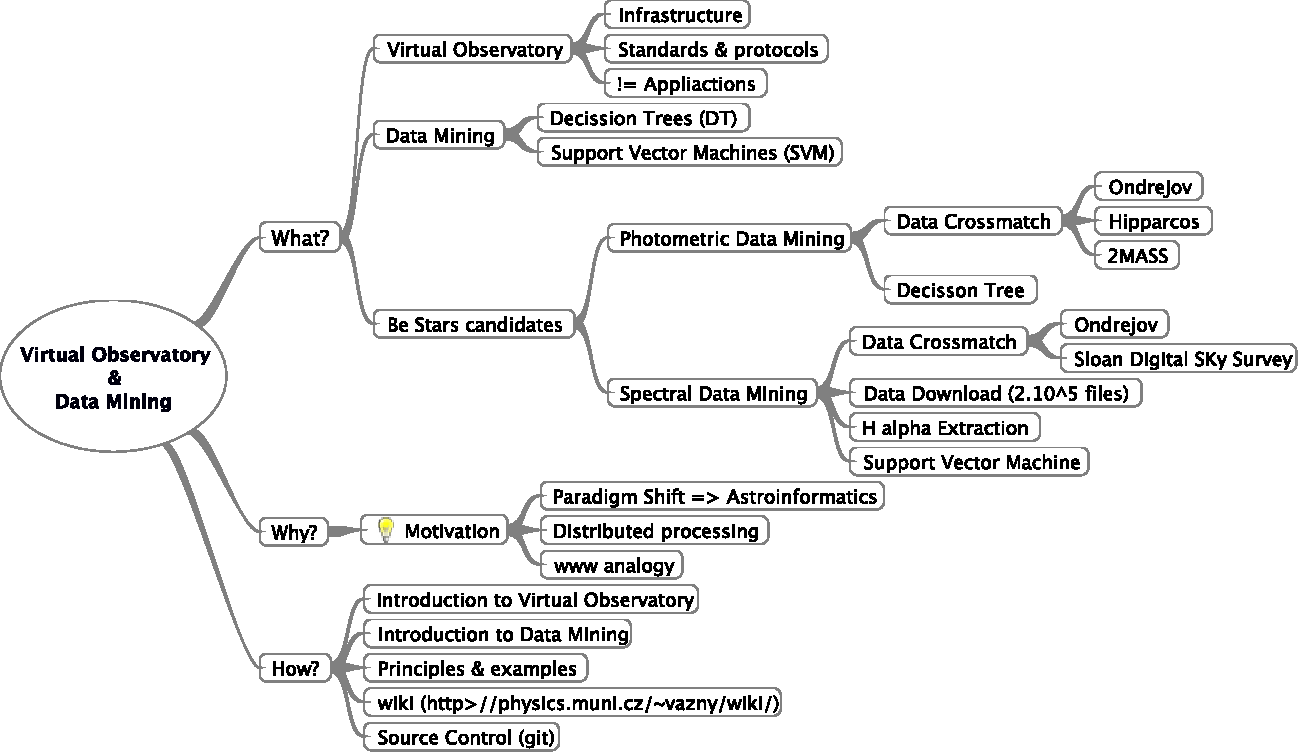
\includegraphics[width=1.0\textwidth]{mainAll}    
  \end{center}
\end{frame}
\end{section}

\begin{section}{What}
  \begin{frame}\frametitle{What is the target of this work?}
  \begin{center}
    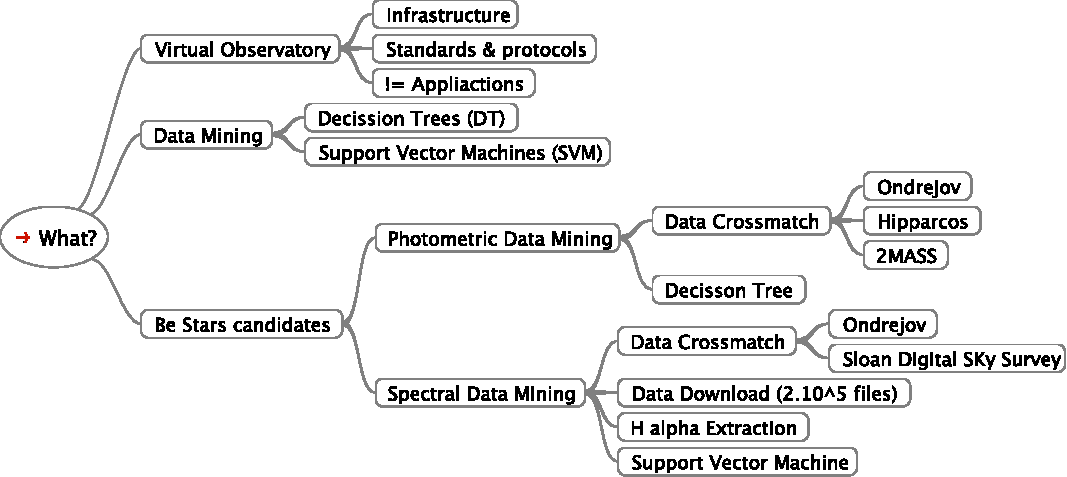
\includegraphics[width=1.0\textwidth]{what}    
  \end{center}
\end{frame}

\begin{frame}\frametitle{Photometric Data Mining}
  \begin{itemize}
  \item \textbf{Be stars Vs B stars Data Mining }
    
    \url{http://physics.muni.cz/~vazny/wiki/index.php/Dm_B_vs_BE}
  \item \textbf{Be stars Vs B stars Color Diagram }
    
    \url{http://physics.muni.cz/~vazny/wiki/index.php/BeColorColor}
  \end{itemize}
\end{frame}


\end{section}

\begin{section}{Why}
  \begin{frame}\frametitle{What is it interesting?}
  \begin{center}
    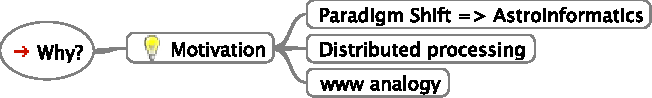
\includegraphics[width=1.0\textwidth]{why}    
  \end{center}
\end{frame}
\end{section}

\begin{section}{How}
  \begin{frame}\frametitle{How is it done?}
  \begin{center}
    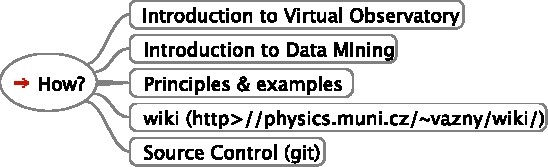
\includegraphics[width=1.0\textwidth]{how}    
  \end{center}
\end{frame}

\begin{frame}[containsverbatim]\frametitle{Example: Reading FITS file}
\begin{lstlisting}[language=SQL]
In [1]: import pyfits
In [2]: hdulist = pyfits.open('spSpec-53237-1886-248.fit')
In [3]: hdulist.info()
Filename: spSpec-53237-1886-248.fit
No.    Name         Type      Cards   Dimensions   Format
0    PRIMARY     PrimaryHDU     213  (3874, 5)     float32
1                BinTableHDU     54  6R x 23C      [1E, 1E, ...
2                BinTableHDU     54  44R x 23C     [1E, 1E, ...
3                BinTableHDU     18  1R x 5C       [1E, 1E, ...
4                BinTableHDU     32  53R x 12C     [1J, 1J, ...
5                BinTableHDU     26  36R x 9C      [19A, 1E, ...
6                BinTableHDU     14  3874R x 3C    [1J, 1J, 1E]
\end{lstlisting}
\end{frame}

\begin{frame}\frametitle{It is more than thesis}
  \begin{itemize}
  \item \textbf{Wiki Documentation}

    \url{http://physics.muni.cz/~vazny/wiki/index.php/Diploma_work}
  \item \textbf{Source Control (Git)}

    \url{https://github.com/astar/diplomaWork}

  \end{itemize}
\end{frame}
\end{section}


\begin{section}{Conclusion}
\begin{frame}
  \begin{center}
 \huge{Wake up!}

 \bigskip

 \huge Q \& A    
  \end{center}
\end{frame}
\end{section}



\end{document}


